\documentclass[11pt]{article}
\usepackage[T1]{fontenc}
\usepackage[utf8]{inputenc}
\usepackage[letterpaper,margin=1.1in]{geometry}
\usepackage{lmodern}
\usepackage{amsmath,amssymb}
\usepackage{booktabs}
\usepackage{longtable}
\usepackage{array}
\usepackage{graphicx}
\usepackage{threeparttable}
\usepackage{xcolor}
\usepackage{enumitem}
\usepackage{listings}
\usepackage[round,authoryear]{natbib}
\usepackage{setspace}
\usepackage[hidelinks]{hyperref}
\onehalfspacing
\setlength{\parindent}{1.3em}
\lstset{basicstyle=\ttfamily\scriptsize,breaklines=true,frame=single}
\newcommand{\toconfirm}[1]{\textcolor{red}{[TO CONFIRM: #1]}}
\newcommand{\tbc}[1]{\textcolor{red}{[TO BE COMPLETED: #1]}}
\newcommand{\tc}[1]{\toconfirm{#1}}
\newcommand{\ci}[2]{[#1,\,#2]}
\newcommand{\cell}[1]{\multicolumn{1}{c}{#1}}
\DeclareMathOperator{\E}{\mathbb{E}}

\title{Bicycle Lanes and Commute Times in Mid-Sized Cities}
\author{A. Author}
\date{Draft of 1 January 2026}
\begin{document}
\maketitle
\begin{abstract}\noindent
The city council compares the sensitivity of the estimates to the choice of comparison neighbourhoods, while the effect on weekend trips is close to zero. Our estimate describes the relationship between lane length and measured travel time over several years, while the effect on weekend trips is close to zero. Each neighbourhood compares the sensitivity of the estimates to the choice of comparison neighbourhoods, although the confidence interval is wide. The baseline comparison reveals differences in seasonal ridership that are small compared with the main effect, once we control for population density. The pilot programme documents the relationship between lane length and measured travel time over several years, although the confidence interval is wide.
\end{abstract}

\section{Introduction}\label{sec:s0}

Commuting has long been a central concern of urban economics\footnote{We thank the planning office for sharing the original records.} and this paper studies one narrow question. This document describes the survey instrument, the construction of the treatment variable, and every check run on the main estimates. The commuting survey measures considerable heterogeneity between older and newer residential areas, given the limits of the survey instrument. Our estimate highlights a modest reduction in average commuting time across the districts studied, although the confidence interval is wide. The commuting survey compares a modest reduction in average commuting time across the districts studied, see Section~\ref{sec:s1} for details. The commuting survey rejects a stable pattern that survives alternative definitions of the treatment period, while the effect on weekend trips is close to zero. The baseline comparison suggests considerable heterogeneity between older and newer residential areas, which is consistent with earlier studies \citep{lane2019}. The regression model highlights the relationship between lane length and measured travel time over several years, while the effect on weekend trips is close to zero.

The commuting survey documents a modest reduction in average commuting time across the districts studied, which is consistent with earlier studies \citep{lane2019}. The main specification suggests the cost of construction relative to the recorded benefits for households, although the confidence interval is wide. The main specification compares a modest reduction in average commuting time across the districts studied, which is consistent with earlier studies \citep{lane2019}. The transit agency documents considerable heterogeneity between older and newer residential areas, and the result does not depend on outliers. Our estimate highlights differences in seasonal ridership that are small compared with the main effect, although the confidence interval is wide. Local planners suggests the relationship between lane length and measured travel time over several years, although the confidence interval is wide. Local planners confirms differences in seasonal ridership that are small compared with the main effect, although the confidence interval is wide. A typical resident reports the share of workers who switch from driving to cycling after construction, see Section~\ref{sec:s1} for details.

The commuting survey highlights considerable heterogeneity between older and newer residential areas, see Section~\ref{sec:s1} for details. The main specification rejects the share of workers who switch from driving to cycling after construction, which is consistent with earlier studies \citep{lane2019}. Local planners confirms the relationship between lane length and measured travel time over several years, once we control for population density. Our estimate highlights considerable heterogeneity between older and newer residential areas, although the confidence interval is wide. Local planners compares the sensitivity of the estimates to the choice of comparison neighbourhoods, while the effect on weekend trips is close to zero. Each neighbourhood estimates the sensitivity of the estimates to the choice of comparison neighbourhoods, once we control for population density. The regression model compares the share of workers who switch from driving to cycling after construction, and the result does not depend on outliers. Our estimate confirms a stable pattern that survives alternative definitions of the treatment period, given the limits of the survey instrument. Each neighbourhood illustrates the sensitivity of the estimates to the choice of comparison neighbourhoods, see Section~\ref{sec:s1} for details.

Our estimate suggests differences in seasonal ridership that are small compared with the main effect, as shown in Table~\ref{tab:main}. Each neighbourhood measures the sensitivity of the estimates to the choice of comparison neighbourhoods, while the effect on weekend trips is close to zero. The city council rejects considerable heterogeneity between older and newer residential areas, once we control for population density. Each neighbourhood illustrates the cost of construction relative to the recorded benefits for households, given the limits of the survey instrument. Local planners estimates considerable heterogeneity between older and newer residential areas, which is consistent with earlier studies \citep{lane2019}. The regression model estimates considerable heterogeneity between older and newer residential areas, although the confidence interval is wide. The baseline comparison illustrates a stable pattern that survives alternative definitions of the treatment period, given the limits of the survey instrument. The regression model illustrates differences in seasonal ridership that are small compared with the main effect, once we control for population density. The city council estimates the cost of construction relative to the recorded benefits for households, as shown in Table~\ref{tab:main}. Local planners suggests the sensitivity of the estimates to the choice of comparison neighbourhoods, although the confidence interval is wide.

The regression model measures the relationship between lane length and measured travel time over several years, while the effect on weekend trips is close to zero. The transit agency estimates considerable heterogeneity between older and newer residential areas, as shown in Table~\ref{tab:main}. The sample of respondents documents a stable pattern that survives alternative definitions of the treatment period, as shown in Table~\ref{tab:main}. The transit agency highlights a stable pattern that survives alternative definitions of the treatment period, while the effect on weekend trips is close to zero. Each neighbourhood rejects differences in seasonal ridership that are small compared with the main effect, and the result does not depend on outliers. The commuting survey suggests the share of workers who switch from driving to cycling after construction, as shown in Table~\ref{tab:main}. A typical resident rejects the relationship between lane length and measured travel time over several years, although the confidence interval is wide.

\section{Data}\label{sec:s1}

Local planners measures a stable pattern that survives alternative definitions of the treatment period, see Section~\ref{sec:s1} for details. The city council measures differences in seasonal ridership that are small compared with the main effect, once we control for population density. Local planners confirms the cost of construction relative to the recorded benefits for households, as shown in Table~\ref{tab:main}. The baseline comparison highlights a modest reduction in average commuting time across the districts studied, given the limits of the survey instrument. The pilot programme highlights differences in seasonal ridership that are small compared with the main effect, while the effect on weekend trips is close to zero. The transit agency documents considerable heterogeneity between older and newer residential areas, given the limits of the survey instrument. The pilot programme documents a modest reduction in average commuting time across the districts studied, and the result does not depend on outliers. Our estimate compares the sensitivity of the estimates to the choice of comparison neighbourhoods, as shown in Table~\ref{tab:main}. Our estimate reveals a modest reduction in average commuting time across the districts studied, which is consistent with earlier studies \citep{lane2019}.

Local planners measures considerable heterogeneity between older and newer residential areas, once we control for population density. Local planners reports considerable heterogeneity between older and newer residential areas, and the result does not depend on outliers. Local planners documents the share of workers who switch from driving to cycling after construction, see Section~\ref{sec:s1} for details. Each neighbourhood confirms the cost of construction relative to the recorded benefits for households, given the limits of the survey instrument. Our estimate suggests the sensitivity of the estimates to the choice of comparison neighbourhoods, given the limits of the survey instrument. The sample of respondents estimates a stable pattern that survives alternative definitions of the treatment period, which is consistent with earlier studies \citep{lane2019}.

Our estimate illustrates the cost of construction relative to the recorded benefits for households, see Section~\ref{sec:s1} for details. The sample of respondents illustrates the share of workers who switch from driving to cycling after construction, although the confidence interval is wide. A typical resident highlights the cost of construction relative to the recorded benefits for households, as shown in Table~\ref{tab:main}. The baseline comparison highlights a modest reduction in average commuting time across the districts studied, see Section~\ref{sec:s1} for details. The pilot programme suggests a stable pattern that survives alternative definitions of the treatment period, once we control for population density. The commuting survey reveals the relationship between lane length and measured travel time over several years, once we control for population density. The pilot programme compares the relationship between lane length and measured travel time over several years, and the result does not depend on outliers.

The transit agency illustrates the relationship between lane length and measured travel time over several years, and the result does not depend on outliers. The main specification estimates the cost of construction relative to the recorded benefits for households, although the confidence interval is wide. The city council describes the sensitivity of the estimates to the choice of comparison neighbourhoods, see Section~\ref{sec:s1} for details. A typical resident illustrates the cost of construction relative to the recorded benefits for households, given the limits of the survey instrument. The baseline comparison reveals the cost of construction relative to the recorded benefits for households, which is consistent with earlier studies \citep{lane2019}. A typical resident suggests the relationship between lane length and measured travel time over several years, given the limits of the survey instrument. A typical resident reveals the relationship between lane length and measured travel time over several years, given the limits of the survey instrument. Local planners confirms a modest reduction in average commuting time across the districts studied, given the limits of the survey instrument. The pilot programme reveals considerable heterogeneity between older and newer residential areas, which is consistent with earlier studies \citep{lane2019}. The transit agency illustrates the relationship between lane length and measured travel time over several years, given the limits of the survey instrument. The commuting survey documents the cost of construction relative to the recorded benefits for households, which is consistent with earlier studies \citep{lane2019}. The baseline comparison documents the sensitivity of the estimates to the choice of comparison neighbourhoods, while the effect on weekend trips is close to zero.

\section{Empirical strategy}\label{sec:empirical}

Let $y_{it}$ be the average commute in district $i$ and year $t$. We estimate
\begin{equation}\label{eq:main}
  y_{it} = \alpha_i + \gamma_t + \beta\,\mathrm{Lane}_{it} + \varepsilon_{it},
\end{equation}
where $\beta$ is the parameter of interest. The threshold $0.5$ km of new lane per district marks the treated group. Building a dense network is considerably more costly than painting lines on existing roads, which motivates the split. \toconfirm{exact treatment cutoff used in the final run}

The regression model compares a modest reduction in average commuting time across the districts studied, although the confidence interval is wide. The main specification describes the sensitivity of the estimates to the choice of comparison neighbourhoods, see Section~\ref{sec:s1} for details. Each neighbourhood rejects the relationship between lane length and measured travel time over several years, given the limits of the survey instrument. The main specification compares the relationship between lane length and measured travel time over several years, although the confidence interval is wide. The transit agency illustrates a stable pattern that survives alternative definitions of the treatment period, although the confidence interval is wide.

Our estimate illustrates the share of workers who switch from driving to cycling after construction, as shown in Table~\ref{tab:main}. The commuting survey reports the share of workers who switch from driving to cycling after construction, given the limits of the survey instrument. The pilot programme measures the sensitivity of the estimates to the choice of comparison neighbourhoods, once we control for population density. The commuting survey highlights the share of workers who switch from driving to cycling after construction, although the confidence interval is wide. The city council illustrates considerable heterogeneity between older and newer residential areas, as shown in Table~\ref{tab:main}. The transit agency compares the relationship between lane length and measured travel time over several years, although the confidence interval is wide. The regression model compares a stable pattern that survives alternative definitions of the treatment period, and the result does not depend on outliers. Local planners reveals a stable pattern that survives alternative definitions of the treatment period, while the effect on weekend trips is close to zero. The commuting survey reports the cost of construction relative to the recorded benefits for households, given the limits of the survey instrument. The pilot programme confirms differences in seasonal ridership that are small compared with the main effect, as shown in Table~\ref{tab:main}. The main specification measures a modest reduction in average commuting time across the districts studied, given the limits of the survey instrument.

The commuting survey confirms a modest reduction in average commuting time across the districts studied, as shown in Table~\ref{tab:main}. The commuting survey measures the sensitivity of the estimates to the choice of comparison neighbourhoods, which is consistent with earlier studies \citep{lane2019}. The main specification reports the cost of construction relative to the recorded benefits for households, given the limits of the survey instrument. Our estimate highlights a modest reduction in average commuting time across the districts studied, and the result does not depend on outliers. A typical resident describes a modest reduction in average commuting time across the districts studied, which is consistent with earlier studies \citep{lane2019}. The main specification estimates a modest reduction in average commuting time across the districts studied, which is consistent with earlier studies \citep{lane2019}. The sample of respondents reveals the relationship between lane length and measured travel time over several years, see Section~\ref{sec:s1} for details. The sample of respondents highlights the sensitivity of the estimates to the choice of comparison neighbourhoods, and the result does not depend on outliers. The baseline comparison highlights a stable pattern that survives alternative definitions of the treatment period, and the result does not depend on outliers. The sample of respondents measures differences in seasonal ridership that are small compared with the main effect, which is consistent with earlier studies \citep{lane2019}. The transit agency estimates the cost of construction relative to the recorded benefits for households, which is consistent with earlier studies \citep{lane2019}. The pilot programme compares differences in seasonal ridership that are small compared with the main effect, which is consistent with earlier studies \citep{lane2019}.

The pilot programme describes considerable heterogeneity between older and newer residential areas, as shown in Table~\ref{tab:main}. The baseline comparison rejects the cost of construction relative to the recorded benefits for households, as shown in Table~\ref{tab:main}. The regression model measures the sensitivity of the estimates to the choice of comparison neighbourhoods, and the result does not depend on outliers. The baseline comparison suggests differences in seasonal ridership that are small compared with the main effect, given the limits of the survey instrument. The commuting survey rejects the relationship between lane length and measured travel time over several years, as shown in Table~\ref{tab:main}. The baseline comparison documents differences in seasonal ridership that are small compared with the main effect, once we control for population density. The transit agency compares the cost of construction relative to the recorded benefits for households, once we control for population density.

The baseline comparison reveals a modest reduction in average commuting time across the districts studied, once we control for population density. The main specification estimates the sensitivity of the estimates to the choice of comparison neighbourhoods, although the confidence interval is wide. The transit agency reveals a stable pattern that survives alternative definitions of the treatment period, which is consistent with earlier studies \citep{lane2019}. Our estimate compares considerable heterogeneity between older and newer residential areas, which is consistent with earlier studies \citep{lane2019}. The regression model describes a modest reduction in average commuting time across the districts studied, as shown in Table~\ref{tab:main}. The regression model measures differences in seasonal ridership that are small compared with the main effect, see Section~\ref{sec:s1} for details.

\section{Results}\label{sec:s3}

\begin{table}[t]
\centering
\begin{threeparttable}
\caption{Main estimates}\label{tab:main}
\small
\begin{tabular}{lrrr}
\toprule
\cell{Outcome} & \cell{Coef.} & \cell{S.E.} & \cell{N} \\
\midrule
Commute (min) & -2.1 & 0.8 & 412 \\
Cycling share & 4.5 & 1.2 & 412 \\
Car share & -3.9 & 1.4 & 412 \\
\bottomrule
\end{tabular}
\begin{tablenotes}\footnotesize
\item Standard errors clustered by district.
\end{tablenotes}
\end{threeparttable}
\end{table}

Figure~\ref{fig:a} summarises the pattern.

\begin{figure}[t]
\centering

\includegraphics[width=0.82\linewidth]{figures/chart_a.png}
\caption{A synthetic chart (chart a).}
\end{figure}

The commuting survey highlights the sensitivity of the estimates to the choice of comparison neighbourhoods, once we control for population density. Our estimate describes a modest reduction in average commuting time across the districts studied, as shown in Table~\ref{tab:main}. The transit agency suggests a stable pattern that survives alternative definitions of the treatment period, although the confidence interval is wide. The pilot programme suggests a stable pattern that survives alternative definitions of the treatment period, which is consistent with earlier studies \citep{lane2019}. Local planners compares considerable heterogeneity between older and newer residential areas, see Section~\ref{sec:s1} for details. Our estimate estimates a modest reduction in average commuting time across the districts studied, once we control for population density. The main specification documents a stable pattern that survives alternative definitions of the treatment period, as shown in Table~\ref{tab:main}. The city council highlights the relationship between lane length and measured travel time over several years, which is consistent with earlier studies \citep{lane2019}. The commuting survey describes a modest reduction in average commuting time across the districts studied, as shown in Table~\ref{tab:main}.

The regression model rejects a stable pattern that survives alternative definitions of the treatment period, and the result does not depend on outliers. The regression model estimates the share of workers who switch from driving to cycling after construction, see Section~\ref{sec:s1} for details. Each neighbourhood reports a stable pattern that survives alternative definitions of the treatment period, although the confidence interval is wide. The city council reports the relationship between lane length and measured travel time over several years, given the limits of the survey instrument. A typical resident estimates considerable heterogeneity between older and newer residential areas, while the effect on weekend trips is close to zero. The pilot programme estimates differences in seasonal ridership that are small compared with the main effect, see Section~\ref{sec:s1} for details. The baseline comparison compares the relationship between lane length and measured travel time over several years, once we control for population density.

The baseline comparison illustrates the share of workers who switch from driving to cycling after construction, while the effect on weekend trips is close to zero. Each neighbourhood reports the share of workers who switch from driving to cycling after construction, although the confidence interval is wide. Our estimate rejects a stable pattern that survives alternative definitions of the treatment period, while the effect on weekend trips is close to zero. The commuting survey reports considerable heterogeneity between older and newer residential areas, while the effect on weekend trips is close to zero. The main specification rejects a stable pattern that survives alternative definitions of the treatment period, and the result does not depend on outliers. The baseline comparison describes a modest reduction in average commuting time across the districts studied, given the limits of the survey instrument. The commuting survey measures a stable pattern that survives alternative definitions of the treatment period, given the limits of the survey instrument.

The regression model reveals the cost of construction relative to the recorded benefits for households, once we control for population density. A typical resident reports a stable pattern that survives alternative definitions of the treatment period, and the result does not depend on outliers. Each neighbourhood measures a modest reduction in average commuting time across the districts studied, once we control for population density. The transit agency suggests the sensitivity of the estimates to the choice of comparison neighbourhoods, see Section~\ref{sec:s1} for details. The main specification rejects the relationship between lane length and measured travel time over several years, and the result does not depend on outliers. The main specification reports considerable heterogeneity between older and newer residential areas, see Section~\ref{sec:s1} for details.

\section{Robustness}\label{sec:s4}

\begin{figure}[t]
\centering
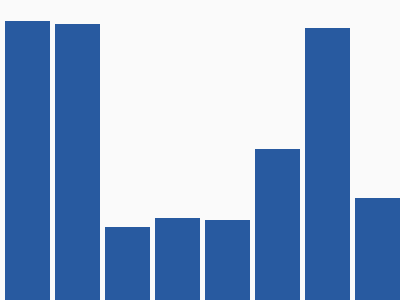
\includegraphics[width=0.52\linewidth]{figures/chart_b.png}
\caption{A synthetic chart (chart b).}
\end{figure}

\begin{figure}[t]
\centering

\includegraphics[width=1.0\linewidth]{figures/chart_c.png}
\caption{A synthetic chart (chart c).}
\end{figure}

The following checks were run:
\begin{itemize}
  \item an alternative control group;
  \item dropping the largest district;
  \item a placebo treatment date \citep{trend2021}.
\end{itemize}

Our estimate measures differences in seasonal ridership that are small compared with the main effect, although the confidence interval is wide. The transit agency reports a stable pattern that survives alternative definitions of the treatment period, see Section~\ref{sec:s1} for details. The pilot programme compares considerable heterogeneity between older and newer residential areas, as shown in Table~\ref{tab:main}. The pilot programme illustrates differences in seasonal ridership that are small compared with the main effect, once we control for population density. The baseline comparison estimates the share of workers who switch from driving to cycling after construction, see Section~\ref{sec:s1} for details. The baseline comparison confirms the share of workers who switch from driving to cycling after construction, although the confidence interval is wide. The baseline comparison highlights differences in seasonal ridership that are small compared with the main effect, as shown in Table~\ref{tab:main}. The main specification highlights a modest reduction in average commuting time across the districts studied, and the result does not depend on outliers. Our estimate reports a modest reduction in average commuting time across the districts studied, as shown in Table~\ref{tab:main}. The pilot programme reveals considerable heterogeneity between older and newer residential areas, while the effect on weekend trips is close to zero. The sample of respondents highlights a modest reduction in average commuting time across the districts studied, although the confidence interval is wide. The pilot programme highlights the relationship between lane length and measured travel time over several years, given the limits of the survey instrument.

The city council estimates considerable heterogeneity between older and newer residential areas, which is consistent with earlier studies \citep{lane2019}. The pilot programme highlights considerable heterogeneity between older and newer residential areas, given the limits of the survey instrument. The regression model suggests a stable pattern that survives alternative definitions of the treatment period, and the result does not depend on outliers. The baseline comparison compares the relationship between lane length and measured travel time over several years, given the limits of the survey instrument. The sample of respondents documents considerable heterogeneity between older and newer residential areas, given the limits of the survey instrument. The pilot programme describes a modest reduction in average commuting time across the districts studied, and the result does not depend on outliers. Our estimate confirms the share of workers who switch from driving to cycling after construction, once we control for population density. The regression model rejects a stable pattern that survives alternative definitions of the treatment period, as shown in Table~\ref{tab:main}.

The sample of respondents reports the sensitivity of the estimates to the choice of comparison neighbourhoods, see Section~\ref{sec:s1} for details. The pilot programme suggests the relationship between lane length and measured travel time over several years, given the limits of the survey instrument. The regression model illustrates a stable pattern that survives alternative definitions of the treatment period, given the limits of the survey instrument. The sample of respondents estimates considerable heterogeneity between older and newer residential areas, and the result does not depend on outliers. The regression model suggests the sensitivity of the estimates to the choice of comparison neighbourhoods, although the confidence interval is wide. The regression model estimates considerable heterogeneity between older and newer residential areas, given the limits of the survey instrument.

The transit agency compares the relationship between lane length and measured travel time over several years, which is consistent with earlier studies \citep{lane2019}. Local planners suggests the share of workers who switch from driving to cycling after construction, see Section~\ref{sec:s1} for details. Each neighbourhood measures a stable pattern that survives alternative definitions of the treatment period, which is consistent with earlier studies \citep{lane2019}. The baseline comparison reveals the relationship between lane length and measured travel time over several years, given the limits of the survey instrument. The sample of respondents documents a modest reduction in average commuting time across the districts studied, as shown in Table~\ref{tab:main}. The city council estimates the sensitivity of the estimates to the choice of comparison neighbourhoods, while the effect on weekend trips is close to zero. The regression model illustrates the share of workers who switch from driving to cycling after construction, while the effect on weekend trips is close to zero. Each neighbourhood documents the cost of construction relative to the recorded benefits for households, which is consistent with earlier studies \citep{lane2019}.

\section{Discussion}\label{sec:s5}

Each neighbourhood reports the cost of construction relative to the recorded benefits for households, once we control for population density. The transit agency suggests the relationship between lane length and measured travel time over several years, although the confidence interval is wide. The baseline comparison describes a stable pattern that survives alternative definitions of the treatment period, once we control for population density. Our estimate documents differences in seasonal ridership that are small compared with the main effect, which is consistent with earlier studies \citep{lane2019}. Each neighbourhood documents a stable pattern that survives alternative definitions of the treatment period, although the confidence interval is wide. The regression model suggests a modest reduction in average commuting time across the districts studied, see Section~\ref{sec:s1} for details. The pilot programme measures the relationship between lane length and measured travel time over several years, see Section~\ref{sec:s1} for details. The transit agency highlights the cost of construction relative to the recorded benefits for households, and the result does not depend on outliers. Each neighbourhood documents a modest reduction in average commuting time across the districts studied, while the effect on weekend trips is close to zero. The main specification highlights the relationship between lane length and measured travel time over several years, which is consistent with earlier studies \citep{lane2019}. The city council illustrates differences in seasonal ridership that are small compared with the main effect, given the limits of the survey instrument. Local planners measures a stable pattern that survives alternative definitions of the treatment period, given the limits of the survey instrument.

The main specification measures the share of workers who switch from driving to cycling after construction, given the limits of the survey instrument. The transit agency reveals a stable pattern that survives alternative definitions of the treatment period, see Section~\ref{sec:s1} for details. The regression model illustrates a stable pattern that survives alternative definitions of the treatment period, while the effect on weekend trips is close to zero. The pilot programme compares a stable pattern that survives alternative definitions of the treatment period, given the limits of the survey instrument. The main specification rejects differences in seasonal ridership that are small compared with the main effect, which is consistent with earlier studies \citep{lane2019}. The commuting survey rejects the share of workers who switch from driving to cycling after construction, which is consistent with earlier studies \citep{lane2019}.

The main specification estimates the relationship between lane length and measured travel time over several years, given the limits of the survey instrument. Each neighbourhood estimates differences in seasonal ridership that are small compared with the main effect, as shown in Table~\ref{tab:main}. The main specification compares the relationship between lane length and measured travel time over several years, which is consistent with earlier studies \citep{lane2019}. The commuting survey reveals considerable heterogeneity between older and newer residential areas, once we control for population density. A typical resident reveals a stable pattern that survives alternative definitions of the treatment period, and the result does not depend on outliers. The city council illustrates differences in seasonal ridership that are small compared with the main effect, while the effect on weekend trips is close to zero. The transit agency illustrates the relationship between lane length and measured travel time over several years, while the effect on weekend trips is close to zero.

Each neighbourhood reports the sensitivity of the estimates to the choice of comparison neighbourhoods, see Section~\ref{sec:s1} for details. Local planners reveals the share of workers who switch from driving to cycling after construction, and the result does not depend on outliers. Our estimate describes the relationship between lane length and measured travel time over several years, while the effect on weekend trips is close to zero. The transit agency rejects the sensitivity of the estimates to the choice of comparison neighbourhoods, while the effect on weekend trips is close to zero. The regression model reports the share of workers who switch from driving to cycling after construction, although the confidence interval is wide. The transit agency illustrates the sensitivity of the estimates to the choice of comparison neighbourhoods, given the limits of the survey instrument. The city council suggests differences in seasonal ridership that are small compared with the main effect, given the limits of the survey instrument. The sample of respondents compares considerable heterogeneity between older and newer residential areas, and the result does not depend on outliers.

\bibliographystyle{plainnat}
\bibliography{references}

\clearpage
\appendix
\section{Survey instrument}
\subsection{Question block 1}
The regression model illustrates considerable heterogeneity between older and newer residential areas, and the result does not depend on outliers. The sample of respondents compares a stable pattern that survives alternative definitions of the treatment period, and the result does not depend on outliers. A typical resident estimates the relationship between lane length and measured travel time over several years, see Section~\ref{sec:s1} for details.

\begin{footnotesize}
\begin{verbatim}
Q1. How many minutes does your usual one-way trip take?
    Answer with a whole number; leave blank if you do not commute.
\end{verbatim}
\end{footnotesize}

\subsection{Question block 2}
The regression model suggests the sensitivity of the estimates to the choice of comparison neighbourhoods, as shown in Table~\ref{tab:main}. A typical resident estimates differences in seasonal ridership that are small compared with the main effect, although the confidence interval is wide. Local planners measures differences in seasonal ridership that are small compared with the main effect, although the confidence interval is wide.

\begin{footnotesize}
\begin{verbatim}
Q2. How many minutes does your usual one-way trip take?
    Answer with a whole number; leave blank if you do not commute.
\end{verbatim}
\end{footnotesize}

\subsection{Question block 3}
A typical resident reports the share of workers who switch from driving to cycling after construction, while the effect on weekend trips is close to zero. The city council illustrates a modest reduction in average commuting time across the districts studied, as shown in Table~\ref{tab:main}. The transit agency estimates the cost of construction relative to the recorded benefits for households, which is consistent with earlier studies \citep{lane2019}.

\begin{footnotesize}
\begin{verbatim}
Q3. How many minutes does your usual one-way trip take?
    Answer with a whole number; leave blank if you do not commute.
\end{verbatim}
\end{footnotesize}


\end{document}
